% =====================================================================
%  Material suplementario
%  Compila por separado. Las referencias cruzadas al articulo principal
%  se escriben a mano porque son dos documentos distintos.
% =====================================================================
\title{Material suplementario\\
       \large Hasta dónde permite decidir la estructura de una serie,
       y por qué ahí se detiene}
\author{Jorge Andres Pe\~na Araya \and Esther Segura P\'erez}
\date{Universidad Nacional Aut\'onoma de M\'exico (UNAM)}
\decimalpoint
\maketitle

\renewcommand{\thetable}{S\arabic{table}}
\renewcommand{\thefigure}{S\arabic{figure}}
\renewcommand{\thesection}{S\arabic{section}}
\setcounter{section}{0}

\noindent
Este documento reúne el material de respaldo del artículo: la composición del vector de
características, la validación del benchmark, el desglose por modelo y frecuencia, la
configuración con la que se ejecutó cada modelo y el detalle del entorno de cómputo.
Nada de lo que sigue es necesario para seguir el argumento; todo es necesario para
reproducirlo.

\section{Composición del vector de características y validaciones}

Los elementos de esta sección se citan desde el artículo principal.

\begin{table}[htbp]
\centering
\caption{Familias de características estructurales.}
\label{tab:familias}
\begin{tabular}{p{0.30\linewidth}p{0.62\linewidth}}
\toprule
\textbf{Familia} & \textbf{Descriptores} \\
\midrule
Forma de la distribución & Asimetría, curtosis, entropía de Shannon, entropía espectral \\
Irregularidad local      & Proporción de atípicos, puntos de giro, puntos de cambio \\
Complejidad              & Exponente de Hurst, entropía robusta \\
Dependencia temporal     & ACF y PACF en múltiples rezagos, decaimiento de autocorrelación \\
Tendencia                & Pendiente, $R^{2}$ lineal, ganancia cuadrática \\
Estacionalidad (STL)     & Fuerza de tendencia, fuerza de ciclo \\
Frecuencia dominante     & Razón de energía del pico espectral dominante \\
Estacionariedad          & ADF, KPSS, indicador de conflicto entre ambos \\
Primeras diferencias     & Razón de varianzas, asimetría, entropía \\
\bottomrule
\end{tabular}
\end{table}

\begin{table}[htbp]
\centering
\caption{Validación del benchmark Naive2 contra los valores publicados.}
\label{tab:naive2}
\begin{tabular}{lrrr}
\toprule
\textbf{Frecuencia} & \textbf{sMAPE replicado} & \textbf{sMAPE publicado} & \textbf{Diferencia} \\
\midrule
Anual       & 16.342 & 16.342 & $0.000$ \\
Trimestral  & 11.024 & 11.012 & $+0.012$ \\
Mensual     & 14.385 & 14.427 & $-0.042$ \\
Semanal     &  9.161 &  9.161 & $0.000$ \\
Diaria      &  3.045 &  3.045 & $0.000$ \\
Horaria     & 18.616 & 18.383 & $+0.233$ \\
\midrule
\textbf{Global} & \textbf{13.548} & \textbf{13.564} & $\mathbf{-0.016}$ \\
\bottomrule
\end{tabular}
\end{table}



\begin{figure}[htbp]
\centering
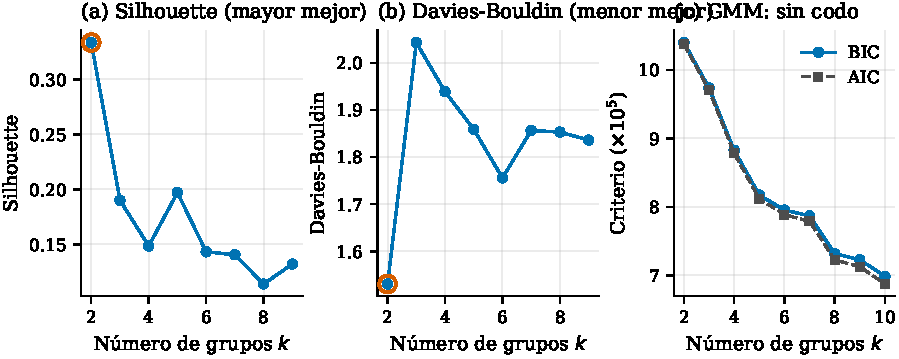
\includegraphics[width=\linewidth]{figuras/fig2_seleccion_k.pdf}
\caption{Selección del número de grupos. (a) Silhouette y (b) Davies-Bouldin
señalan $k=2$ (marcado en naranja). (c) BIC y AIC de los modelos de mezcla
gaussiana decrecen sin codo, lo que no respalda particiones más finas.}
\label{fig:seleccion}
\end{figure}

\begin{figure}[htbp]
\centering
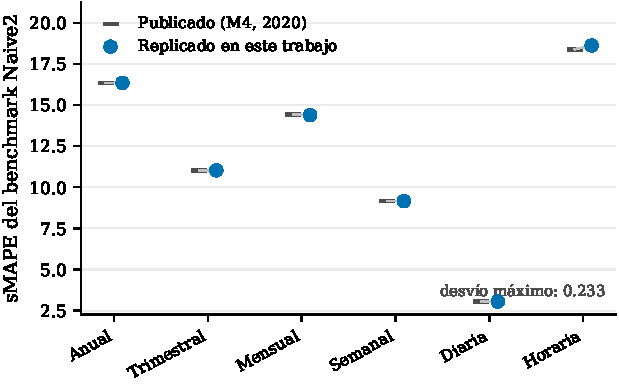
\includegraphics[width=0.62\linewidth]{figuras/fig9_validacion_naive2.pdf}
\caption{Benchmark Naive2 replicado frente al publicado por la competencia. Las
frecuencias con $m=1$ coinciden de forma exacta.}
\label{fig:naive2}
\end{figure}

% =====================================================================

\section{Fallos catastróficos frente a fallos mediocres}\label{sec:extremos}

Cuatro modelos presentan OWA entre 11 y 365, valores que a primera vista sugieren
un desempeño inutilizable. Sus medianas, sin embargo, se ubican entre $0.9$ y
$1.8$: el promedio esta dominado por un número reducido de series
(Cuadro~\ref{tab:extremos}).

\begin{table}[htbp]
\centering
\caption{Modelos cuyo MASE promedio esta dominado por casos extremos. La columna
final cuenta las series con $\mathrm{MASE}>100$ sobre un total de 5{,}773.}
\label{tab:extremos}
\begin{tabular}{lrrr}
\toprule
\textbf{Modelo} & \textbf{MASE medio} & \textbf{MASE mediano} & \textbf{Series extremas} \\
\midrule
ARIMA-NN     & 1{,}782.3 & 1.57 & 3 \\
LSTM         & 289.6     & 2.51 & 32 \\
LSTM-Conv1D  & 136.1     & 2.58 & 21 \\
SARIMA-NN    & 51.8      & 1.37 & 17 \\
Holt         & 7.5       & 1.71 & 118 \\
\bottomrule
\end{tabular}
\end{table}

El mecanismo es una asimetría entre las dos métricas: \textbf{sMAPE esta acotado en
200, MASE no tiene cota superior}. Un pronóstico que diverge queda saturado en el
sMAPE y arrastra sin limite el promedio del MASE. El caso testigo es la serie
\texttt{H366}, donde SARIMA produce sMAPE $=199.99$ ---practicamente el máximo
posible--- y MASE $=127{,}224$; esa única serie explica el total del MASE promedio
de la frecuencia horaria.

De los 118 casos extremos de Holt, 117 son horarios: el modelo extrapola una
tendencia lineal a 48 pasos sobre series con ciclo diario, y diverge.

El caso más llamativo por magnitud es SARIMA-NN en la frecuencia mensual, con
$\mathrm{OWA}=114.82$. La cifra parece descartar el modelo, pero su MASE mediano en esa
frecuencia es $0.83$ ---es decir, \emph{mejor que el benchmark en la serie típica}--- y
el promedio de $236.7$ proviene de 13 series de 1{,}000. Es el mismo mecanismo de cola
descrito arriba llevado al extremo, y es la razón por la que la
Sección~6.5 del artículo lo ubica cuarto por rangos pese a figurar último por OWA.

La implicación práctica es directa. Para uso productivo, un modelo que falla de
forma catastrófica en el 0.3\,\% de los casos es preferible \emph{menos} que uno
consistentemente mediocre, porque el fallo no es detectable a priori. Al reportar
MASE promedio conviene acompañarlo de la mediana y del conteo de casos extremos.

\paragraph{Un tercer modo de fallo: la incapacidad estructural.} Los casos
anteriores comparten que el modelo funciona bien de forma típica y se descontrola en
pocas series. LightGBM, con OWA global $=1.702$, el peor del banco, responde a un
mecanismo distinto que conviene separar porque tiene otra lectura. Su fallo no está en
la cola sino en el centro de la distribución, y no es uniforme entre frecuencias: en
mensual y trimestral su sMAPE mediano es $9.9$ y $9.2$, competitivo; en anual y horaria
es $30.7$ y $20.4$, muy por detrás del benchmark. La explicación es una propiedad del
modelo y no de su implementación: \textbf{un ensamble de árboles predice promedios de
hojas y por construcción no puede extrapolar fuera del rango observado}.

La evidencia es directa. En la frecuencia anual, cuya serie mediana tiene apenas 29
observaciones, LightGBM emite un pronóstico \emph{plano} ---coeficiente de variación
menor a $10^{-3}$ a lo largo del horizonte--- en el 95.7\,\% de las series, frente al
12.5\,\% de ARIMA. Con tan pocas filas de entrenamiento tras construir los rezagos, los
árboles no encuentran particiones con soporte suficiente y colapsan a una constante
próxima a la media de la muestra. Naive2 también es constante en esa frecuencia, pero
lo es \emph{en el último valor}, que sobre series con tendencia es una constante mucho
mejor. En la frecuencia horaria el pronóstico no es plano pero sí amortiguado: su
coeficiente de variación mediano es $0.038$ contra $0.201$ del benchmark, es decir que
reproduce el ciclo diario con una quinta parte de la amplitud que la serie realmente
tiene.

Esto no invalida la evaluación: LightGBM se ajustó con búsqueda aleatoria sobre el
mismo espacio de hiperparámetros que los demás métodos de aprendizaje automático
(material suplementario), y su resultado es el que corresponde a aplicar un
ensamble de árboles a series cortas con tendencia y a horizontes largos con
estacionalidad marcada. Reportarlo tiene valor precisamente por eso: \textbf{la
distinción entre un modelo mal ajustado y un modelo estructuralmente inadecuado para
una familia de series es exactamente el tipo de heterogeneidad que una regla de
decisión condicionada por estructura debería capturar}, y explica por qué LightGBM
nunca aparece en los conjuntos que la Sección~7.3 del artículo selecciona para anual
u horaria.


\begin{table}[htbp]
\centering
\caption{Sensibilidad al número de estratos de complejidad. La columna de ventaja es
la diferencia de OWA entre la regla B y la regla C; valores positivos favorecen al
índice.}
\label{tab:estratos}
\begin{tabular}{crrcr}
\toprule
\textbf{Estratos} & \textbf{OWA de C} & \textbf{Ventaja sobre B} &
\textbf{C mejor en} & \textbf{$p$} \\
\midrule
\textbf{2} & \textbf{0.8835} & \textbf{$+0.0306$} & \textbf{30/30} & $1.9\times10^{-9}$ \\
3 & 0.8898 & $+0.0243$ & 30/30 & $1.9\times10^{-9}$ \\
4 & 0.8853 & $+0.0287$ & 30/30 & $1.9\times10^{-9}$ \\
5 & 0.8918 & $+0.0223$ & 29/30 & $3.8\times10^{-6}$ \\
\bottomrule
\end{tabular}
\end{table}


\begin{table}[htbp]
\centering
\caption{Estabilidad del índice de complejidad ante perturbaciones, sobre 300 series
por frecuencia. Cada celda es el porcentaje de series que cruza el corte de la mediana
al recalcular el índice sobre la serie perturbada, y entre paréntesis la correlación de
Spearman entre el índice original y el perturbado. El corte se fija siempre con el
índice original.}
\label{tab:estabilidad}
% Siete columnas no caben a 11pt: a cuerpo normal se sale 38pt del margen.
\small
\setlength{\tabcolsep}{4.5pt}
\begin{tabular}{lrrrrrr}
\toprule
\textbf{Perturbación} & \textbf{Anual} & \textbf{Trimestral} & \textbf{Mensual} & \textbf{Semanal} & \textbf{Diaria} & \textbf{Horaria} \\
\midrule
Ruido 1\,\% & 2.0 (0.990) & 1.3 (0.997) & 1.3 (0.998) & 1.7 (0.997) & 1.7 (0.994) & 0.3 (0.999) \\
Ruido 2\,\% & 3.7 (0.987) & 1.0 (0.997) & 2.0 (0.997) & 2.7 (0.996) & 3.0 (0.993) & 1.0 (0.996) \\
Ruido 5\,\% & 6.3 (0.979) & 2.7 (0.989) & 3.3 (0.993) & 5.8 (0.993) & 8.0 (0.984) & 2.7 (0.990) \\
\midrule
Historia 75\,\% & 16.3 (0.899) & 17.7 (0.865) & 26.0 (0.800) & 14.3 (0.841) & 28.3 (0.657) & 10.7 (0.960) \\
Historia 50\,\% & 33.1 (0.701) & 37.3 (0.642) & 37.7 (0.641) & 28.9 (0.577) & 41.3 (0.278) & 17.3 (0.939) \\
\bottomrule
\end{tabular}
\end{table}


% =====================================================================
\section{Por qué fracasa el clasificador}\label{sec:clasificador}
% =====================================================================

La Sección~7.2 del artículo reporta que la política E ---un bosque aleatorio que
predice \emph{cuál} modelo gana en cada serie--- queda en OWA $1.4927$, peor que no
enrutar, y atribuye el fracaso a la inestabilidad de la etiqueta. La explicación es
plausible y no es la única: hay al menos cuatro candidatas, las cuatro predicen el mismo
fracaso y se distinguen por lo que ocurre al corregir cada una. Esta sección las pone a
prueba sobre las mismas 30 particiones, el mismo banco, el mismo bosque de 300 árboles y
la misma semilla, de modo que la fila E del Cuadro~\ref{tab:clasificador} reproduce
dígito a dígito el valor publicado.

\paragraph{El desbalance de clases no es la causa.} La etiqueta reparte 27 modelos con
entropía normalizada de $0.911$ y una clase mayoritaria del 13.5\,\%: el problema no es
degenerado. Reentrenar con pesos de clase balanceados baja la \emph{media} de $1.4927$ a
$1.0453$, pero sube la \emph{mediana} de $0.9851$ a $1.0233$. No arregla la partición
típica ---la empeora---; lo único que hace es cortar la cola, porque el máximo entre
particiones pasa de $15.21$ a $1.18$. El desbalance explica la varianza del fracaso, no
el fracaso.

\paragraph{La causa dominante es la asimetría de los costos.} La clasificación minimiza
la pérdida $0$--$1$: equivocarse de modelo cuesta lo mismo siempre. Pero elegir el
segundo mejor cuesta milésimas y elegir uno que diverge cuesta órdenes de magnitud
(Sección~\ref{sec:extremos}). El daño resulta, en efecto, concentrado: el 0.1\,\% peor
de las series aporta el 22.3\,\% del exceso de OWA sobre la política por frecuencia, el
1\,\% peor el 40.1\,\% y el 5\,\% peor el 67.8\,\%
(Figura~\ref{fig:clasificador}). Descartando de cada política su propio 1\,\% peor, el
clasificador pasa de $1.4927$ a $0.8831$ y deja de ser catastrófico.

El corte decisivo, sin embargo, es correctivo y no descriptivo. Conservando el mismo
bosque y la misma etiqueta ---con todo su ruido--- y cambiando \emph{solo} la regla de
decisión, de quedarse con la clase más probable a minimizar el arrepentimiento esperado
$\sum_c p(c\mid x)\,L[c,m]$, con $L[c,m]$ el arrepentimiento medio de elegir $m$ entre
las series de entrenamiento cuyo ganador es $c$, el OWA pasa de $1.4927$ a
$\mathbf{0.8661}$: mejor que el índice ($0.8835$, en las 30 particiones,
$p=1.9\times10^{-9}$) y mejor que el regresor por modelo ($0.8746$, en 22 de 30,
$p=5.6\times10^{-4}$).

Dos controles descartan las lecturas fáciles. Si se reemplaza $p(c\mid x)$ por la
proporción de entrenamiento ---la misma matriz de costos, sin mirar los atributos--- el
OWA es $0.9165$, que es la regla por frecuencia: la estructura de costos por sí sola no
compra nada, y los atributos aportan $0.0504$ de los $0.0573$ que separan a $E_3$ del
modelo fijo. Y si la matriz se estima una sola vez para todas las frecuencias en lugar de
una por frecuencia, el OWA es $0.8814$, todavía por delante del índice: el resultado no
depende de condicionar por frecuencia.

\paragraph{Las probabilidades están calibradas, y la política E las descarta.} La
exactitud del clasificador es del 18.5\,\% ---40.7\,\% si se admite el top-3--- y su
confianza media es $0.206$, con un error esperado de calibración de $0.023$. El bosque,
dicho de otro modo, \emph{sabe que no sabe}, y la política E tira esa información al
quedarse con la clase más probable. Una regla con abstención ---usar el ganador de la
frecuencia cuando la confianza no llega a $\tau$--- alcanza $0.9016$ con $\tau=0.25$,
absteniéndose en el 77\,\% de las series. Es mejor que no enrutar y muy inferior a
corregir la pérdida: la calibración es aprovechable, pero no es donde está el problema.

\paragraph{La etiqueta sí es casi arbitraria, y aun así no es lo que hunde al OWA.} En el
11.5\,\% de las series el primero y el segundo tienen el \emph{mismo} sMAPE ---modelos
que colapsan al mismo pronóstico--- y en el 24.6\,\% los separa menos del 1\,\%, con
una mediana del 5.9\,\%. La etiqueta es inestable en esa medida, y eso acota la
exactitud alcanzable con independencia del clasificador que se use. Lo que la evidencia
anterior muestra es que la exactitud baja no es lo que produce el $1.49$: con la misma
etiqueta y el mismo bosque, cambiar la regla de decisión basta para llegar a $0.8661$.

\paragraph{Qué corrige esto de la lectura del artículo.} La recomendación de diseño
sobrevive ---predecir el error de cada candidato y quedarse con el menor es robusto;
predecir el ganador y creerle no lo es--- pero su razón cambia. La formulación como
regresión no domina porque la etiqueta sea ruido, sino porque \textbf{codifica la
pérdida}; la clasificación con la pérdida codificada domina a las dos. Conviene además no
leer el 15.0\,\% de $E_3$ junto a las cifras de la Sección~7.3 del artículo: aquel
experimento sortea las particiones de otro modo y tiene por lo tanto otra cota del
oráculo, de manera que sus cifras son comparables dentro de él y no entre experimentos.

\begin{table}[htbp]
\centering
\caption{Las cuatro explicaciones del fracaso del clasificador, puestas a prueba. Todas
las filas comparten las 30 particiones, el banco, el bosque de 300 árboles y la semilla;
la fila E reproduce el valor del Cuadro~5 del artículo. La columna de cierre es la
fracción del hueco entre el modelo fijo ($0.9234$) y el oráculo por serie ($0.5423$).}
\label{tab:clasificador}
\begin{tabular}{llrrrr}
\toprule
& \textbf{Variante} & \textbf{OWA} & \textbf{Mediana} & \textbf{d.e.} & \textbf{Cierra} \\
\midrule
E & Clasificador, clase más probable & 1.4927 & 0.9851 & 2.592 & $-152.2$\,\% \\
\midrule
\multicolumn{6}{@{}l}{\emph{(1) Desbalance de clases}}\\
$E_1$ & Pesos de clase balanceados & 1.0453 & 1.0233 & 0.066 & $-32.0$\,\% \\
\multicolumn{6}{@{}l}{\emph{(2) Costos de error heterogéneos}}\\
$E_2$ & Etiquetas podadas a 10 modelos & 0.9152 & 0.9175 & 0.017 & $2.1$\,\% \\
$E_3$ & Decisión de Bayes con costos & \textbf{0.8661} & 0.8659 & 0.006 & \textbf{15.0}\,\% \\
\multicolumn{6}{@{}l}{\emph{(3) Calibración}}\\
$E_4$ & Abstención bajo $\tau=0.25$ & 0.9016 & 0.8956 & 0.024 & $5.7$\,\% \\
\midrule
\multicolumn{6}{@{}l}{\emph{Controles sobre $E_3$}}\\
 & Sin atributos, solo la proporción & 0.9165 & 0.9151 & 0.007 & $1.8$\,\% \\
 & Matriz única, sin frecuencia & 0.8814 & 0.8808 & 0.008 & $11.0$\,\% \\
\midrule
\multicolumn{6}{@{}l}{\emph{Referencias del Cuadro~5 del artículo}}\\
B & Por frecuencia & 0.9140 & 0.9140 & 0.007 & $2.4$\,\% \\
C & Frecuencia $\times$ índice & 0.8835 & 0.8832 & 0.006 & $10.5$\,\% \\
F & Regresor por modelo & 0.8746 & 0.8730 & 0.014 & $12.8$\,\% \\
\bottomrule
\end{tabular}
\end{table}

\begin{figure}[htbp]
\centering
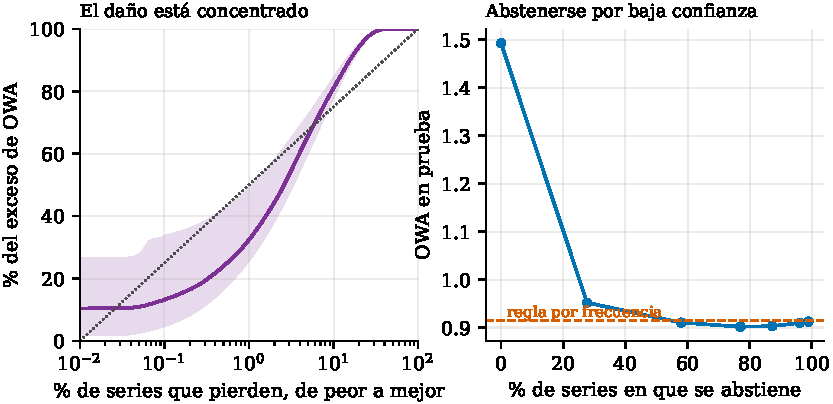
\includegraphics[width=\linewidth]{figuras/fig16_clasificador.pdf}
\caption{Izquierda: fracción del exceso de OWA sobre la política por frecuencia que
aportan las series ordenadas de peor a mejor, dentro de cada partición. La línea es la
mediana de las 30 curvas y la banda el rango intercuartílico; la diagonal punteada sería
un daño repartido por igual. La curva se calcula partición por partición porque agregar
las 30 no es informativo: una sola serie de la partición que se dispara a $15.21$ se
lleva dos tercios del exceso acumulado. Derecha: OWA de la regla con abstención según la
fracción de series en que se abstiene.}
\label{fig:clasificador}
\end{figure}


\section{Validación fuera de M4}\label{sec:m3}
% =====================================================================

Todo el artículo transcurre dentro de M4: el índice se construye con M4, los cortes se
fijan con M4 y las políticas se entrenan y se prueban en mitades de M4. La objeción es
inmediata ---cuánto de todo esto es M4--- y admite una respuesta que no exige reentrenar
nada. La competencia M3 publicó los \emph{pronósticos} de los métodos que compitieron,
serie por serie y horizonte por horizonte (Makridakis y Hibon, 2000; distribuidos en el
paquete \texttt{Mcomp}, ambos citados en el artículo), de modo que el
error por serie y por modelo se reconstruye sin ajustar un solo modelo nuevo. Eso es lo
pertinente cuando la pregunta es si transfiere la \emph{regla} y no si uno sabe entrenar
modelos. Dos de los 24 métodos ---AAM1 y AAM2--- sólo pronosticaron las series
trimestrales y mensuales, y el protocolo exige el banco completo en cada serie: quedan 22
métodos sobre las 3\,003 series, con NAIVE2 dentro del banco y a la vez como denominador
del OWA, igual que naive2 en M4.

Los descriptores se calculan con el mismo código que los calculó sobre M4, y el índice se
\textbf{transfiere}: las medianas de imputación, las medias y escalas del estandarizador y
los pesos de PC1 se estiman en M4 y se aplican a M3 sin reajuste. Eso es lo que hace de
esto una prueba externa y no un reajuste con otro nombre. Dos verificaciones sostienen el
montaje: al rehacer el ajuste sobre M4 el índice recalculado coincide con el guardado con
una diferencia máxima de $5.3\times10^{-15}$, y el OWA reconstruido sobre M3 pone en
primer lugar a THETA (0.8516), el método que mejor se desempeñó en aquella
competencia. Los niveles de OWA de M3 y M4 no son comparables entre sí
---distinto banco, distinto tamaño, distintas frecuencias y distinto oráculo--- y no se
los compara: lo comparable es la estructura, es decir qué afirmaciones se repiten y qué
fracción del hueco hasta el oráculo queda sin recorrer.

\paragraph{El índice transfiere como medida de dificultad.} PC1 explica el 28.1\,\% de la
varianza en M3 contra el 26.9\,\% en M4, y el índice transferido correlaciona $0.995$ con
el que se obtiene reestimando todo dentro de M3: la estructura de covarianza de los 29
descriptores es prácticamente la misma en las dos colecciones. Y ordena por dificultad
igual de bien o mejor: la correlación de Spearman con el sMAPE del ingenuo es $+0.488$ en
M3 contra $+0.410$ en M4, y el primer decil del índice tiene un error de un tercio de la
media de su colección mientras el último casi la duplica, en las dos
(Figura~\ref{fig:m3}c).

\paragraph{Y no transfiere como clave de enrutamiento.} La política C ---estratificar por
frecuencia y por la mediana del índice--- recorre el 10.5\,\% del hueco hasta el oráculo
en M4 y sólo el 1.9\,\% en M3, con ventaja sobre la regla por frecuencia en 22 de 30
particiones ($p=0.028$). Con el índice reestimado dentro de M3 la ventaja baja a 21 de 30
y deja de ser significativa ($p=0.10$), de manera que lo que no transfiere no es el
índice: es que haya algo que ganar estratificando. Esta es la limitación más fuerte que
el trabajo encuentra sobre sí mismo, y conviene enunciarla sin suavizarla: \textbf{el
índice mide la dificultad en las dos colecciones y sólo en una de ellas eso se convierte
en una mejor elección de modelo}.

\paragraph{El margen lo fija el banco, no las series.} La razón no está en las series de
M3 sino en sus métodos. Cinco de los 22 quedan a menos del 5\,\% del mejor ---en M4 sólo
dos de 27 están tan cerca del mejor--- y THETA gana casi en todas partes: apenas 4 de las
8 celdas de la política C eligen algo distinto del ganador global, contra 9 de 12 en M4.
No es que las series de M3 sean más homogéneas; de hecho la etiqueta del oráculo está más
repartida allí (entropía normalizada $0.967$ y clase mayoritaria del 7.5\,\%, contra
$0.911$ y 13.5\,\% en M4). Lo que es más homogéneo es el banco. El enrutamiento sólo puede
comprar algo si los candidatos difieren lo bastante entre sí, y esa es una propiedad del
banco que se elija, no de la colección que se pronostique.

\paragraph{La corrección de la Sección~\ref{sec:clasificador} transfiere, y sin modelos
que divergen.} La política E vuelve a quedar por debajo de la regla por frecuencia, ahora
en 28 de 30 particiones ($p=1.9\times10^{-8}$), y cambiar sólo la regla de decisión ---el
mismo bosque, la misma etiqueta, el arrepentimiento esperado en lugar de la clase más
probable--- la lleva de $0.8725$ a $0.8322$, por delante del índice en 27 de 30
($p=1.7\times10^{-6}$). Importa cómo ocurre: en M3 \emph{ningún} candidato se dispara. El
peor de los 22 métodos queda en OWA $1.022$, mientras que en M4 seis de los 27 modelos
superan el OWA $2$ y el peor llega a $271.8$. La objeción natural a la
Sección~\ref{sec:clasificador} ---que el problema de la pérdida $0$--$1$ se reduce a unos
pocos candidatos catastróficos--- queda así descartada: la asimetría de costos basta para
hundir al clasificador en un banco donde nada diverge.

\paragraph{Lo que no se sostiene fuera de M4.} Que el clasificador con costos le gane al
regresor por modelo es un resultado de M4. En M3 las dos políticas empatan ($0.8322$
contra $0.8293$, 11 de 30 particiones a favor del clasificador, $p=0.29$). La afirmación
que sobrevive al cambio de colección es la más débil de las dos, y es la que conviene
hacer: una vez que la pérdida está codificada, clasificar y regresar llegan al mismo
lugar, y elegir entre ellas es cuestión de conveniencia y no de principio.

\paragraph{El techo es peor afuera.} En M3 la mejor de las políticas deja sin recuperar el
93.3\,\% del hueco entre el modelo fijo y el oráculo por serie; en M4, el 85.0\,\%. El
resultado central del artículo no sólo sobrevive al cambio de colección: es más severo
fuera que dentro, y lo es contra un banco de métodos que no se eligió aquí y en el que
ninguna decisión de este trabajo pudo influir.

\begin{table}[htbp]
\centering
\caption{Las políticas del Cuadro~5 del artículo, repetidas sobre las 3\,003 series de M3
con los pronósticos publicados de 22 métodos y el mismo protocolo de 30 particiones. Los
OWA de los dos bloques \textbf{no} son comparables entre sí ---distinto banco y distinto
oráculo---; lo comparable es la columna de cierre, la fracción del hueco entre el modelo
fijo y el oráculo que cada política recorre. El índice usado en M3 es el de M4,
transferido sin reajuste.}
\label{tab:m3}
\begin{tabular}{llrrrr}
\toprule
& & \multicolumn{2}{c}{\textbf{M4} · 27 modelos}
  & \multicolumn{2}{c}{\textbf{M3} · 22 métodos} \\
\cmidrule(lr){3-4}\cmidrule(lr){5-6}
& \textbf{Política} & \textbf{OWA} & \textbf{Cierra} & \textbf{OWA} & \textbf{Cierra} \\
\midrule
A & Modelo fijo & 0.9234 & --- & 0.8527 & --- \\
B & Por frecuencia & 0.9140 & 2.4\,\% & 0.8492 & 1.0\,\% \\
C & Frecuencia $\times$ índice & 0.8835 & 10.5\,\% & 0.8460 & 1.9\,\% \\
E & Clasificador & 1.4927 & $-152.2$\,\% & 0.8725 & $-5.8$\,\% \\
E$'$ & Clasificador con costos & \textbf{0.8661} & \textbf{15.0}\,\% & 0.8322 & 5.9\,\% \\
F & Regresor por modelo & 0.8746 & 12.8\,\% & \textbf{0.8293} & \textbf{6.7}\,\% \\
D & Oráculo (cota) & 0.5423 & 100\,\% & 0.5078 & 100\,\% \\
\bottomrule
\end{tabular}
\end{table}

\begin{figure}[htbp]
\centering
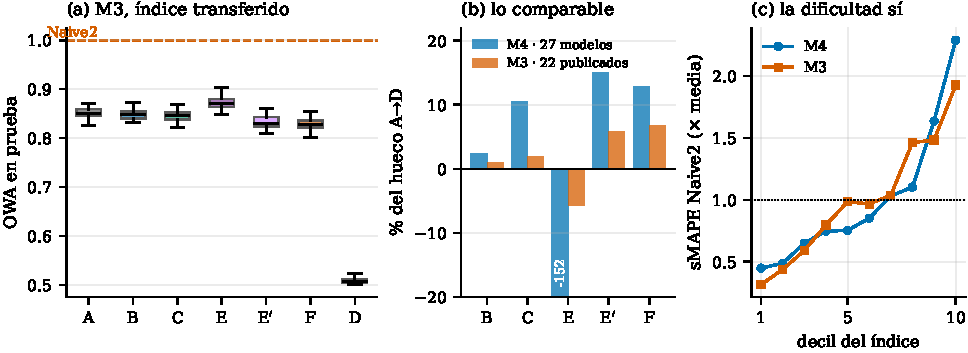
\includegraphics[width=\linewidth]{figuras/fig17_validacion_m3.pdf}
\caption{(a) Las políticas sobre M3, con el índice transferido de M4. (b) La única
comparación legítima entre las dos colecciones: no el OWA sino la fracción del hueco
entre el modelo fijo y el oráculo que recorre cada política; la barra de E en M4 vale
$-152$\,\% y está cortada. (c) Lo que sí transfiere: el sMAPE del ingenuo por decil del
índice, en múltiplos de la media de cada colección.}
\label{fig:m3}
\end{figure}


\appendix
\section{Configuración de los modelos}\label{ap:hiperparametros}
% =====================================================================

El Cuadro~\ref{tab:hiperparametros} detalla la configuración de los 27 modelos.
Los valores no se transcriben de la documentación de las bibliotecas sino de la
configuración registrada en cada corrida, de modo que reflejan lo que
efectivamente se ejecutó. Para los modelos ajustados por búsqueda aleatoria se
indica el espacio de búsqueda y no el valor seleccionado, que difiere entre
series. Las arquitecturas de las redes neuronales se obtuvieron instanciando cada
modelo y leyendo sus capas.

% Tabla de hiperparametros -- generada por tabla_hiperparametros.py
% Requiere: \usepackage{booktabs}, \usepackage{longtable} y \usepackage{array}
% Las columnas van en ragged right: justificado en una columna angosta
% deja huecos y LaTeX lo reporta como underfull hbox.
\begin{longtable}{>{\raggedright\arraybackslash}p{0.21\linewidth}>{\raggedright\arraybackslash}p{0.71\linewidth}}
\caption{Configuración de los 27 modelos evaluados. Los valores provienen de la configuración efectivamente registrada en cada corrida, no de la documentación de las bibliotecas. ``por serie'' indica que el parámetro se selecciona automáticamente para cada serie.}\label{tab:hiperparametros}\\
\toprule
\textbf{Modelo} & \textbf{Configuración} \\
\midrule
\endfirsthead
\toprule
\textbf{Modelo} & \textbf{Configuración} \\
\midrule
\endhead
\bottomrule
\endfoot
\multicolumn{2}{l}{\textit{Referencia}} \\[1mm]
\hspace{.6em}Naive & Repite la última observación \\
\hspace{.6em}Naive estacional & periodo = 4 \\
\addlinespace
\multicolumn{2}{l}{\textit{Estadístico}} \\[1mm]
\hspace{.6em}Suavizado Exponencial & alpha\_optimizado: por serie \\
\hspace{.6em}Holt & alpha\_optimizado: por serie; beta\_optimizado: por serie \\
\hspace{.6em}Holt-Winters & alpha: por serie; beta: por serie; gamma: por serie \\
\hspace{.6em}ARIMA & p\_d\_q: por serie; P\_D\_Q\_m: por serie \\
\hspace{.6em}SARIMA & p\_d\_q: por serie; P\_D\_Q\_m: por serie \\
\hspace{.6em}ETS & alpha: por serie; use\_boxcox = False \\
\addlinespace
\multicolumn{2}{l}{\textit{Aprendizaje automático}} \\[1mm]
\hspace{.6em}Regresión lineal & fit\_intercept = True; tol = 1e-06 \\
\hspace{.6em}LassoLars & Ajustado por serie con RandomizedSearchCV (25 muestras, validación cruzada de 3 pliegues) sobre: alpha $\in$ logspace($-4$, 1, 60); max\_iter $\in$ \{200, 500, 1000, 2000\}; fit\_intercept, positive, precompute \\
\hspace{.6em}Regresión bayesiana & Ajustado por serie con RandomizedSearchCV (25 muestras, validación cruzada de 3 pliegues) sobre: alpha$_1$, alpha$_2$, lambda$_1$, lambda$_2$ $\in$ logspace($-8$, $-2$, 20); tol $\in$ \{1e-6, 1e-5, 1e-4, 1e-3\} \\
\hspace{.6em}Bagging & Ajustado por serie con RandomizedSearchCV (30 muestras, validación cruzada de 3 pliegues) sobre: n\_estimators $\in$ \{50, 100, 200, 300, 500\}; max\_samples y max\_features $\in$ \{0.5, 0.7, 0.9, 1.0\}; bootstrap \\
\hspace{.6em}Random Forest & Ajustado por serie con RandomizedSearchCV (30 muestras, validación cruzada de 3 pliegues) sobre: n\_estimators $\in$ \{50, 100, 200, 300\}; max\_depth $\in$ \{None, 5, 10, 20, 30\}; min\_samples\_split, min\_samples\_leaf; max\_features $\in$ \{sqrt, log2, None\} \\
\hspace{.6em}AdaBoost & Ajustado por serie con RandomizedSearchCV (30 muestras, validación cruzada de 3 pliegues) sobre: n\_estimators $\in$ \{50, 100, 200, 300, 500\}; learning\_rate $\in$ \{0.01, 0.05, 0.1, 0.2, 0.5, 1.0\}; loss $\in$ \{linear, square, exponential\}; profundidad del arbol base $\in$ \{2--6, None\} \\
\hspace{.6em}XGBoost & Ajustado por serie con RandomizedSearchCV (30 muestras, validación cruzada de 3 pliegues) sobre: n\_estimators $\in$ \{100, 200, 300, 500\}; learning\_rate $\in$ \{0.01, 0.05, 0.1, 0.2\}; max\_depth $\in$ \{3, 5, 7, 10\}; subsample y colsample\_bytree $\in$ \{0.6, 0.8, 1.0\} \\
\hspace{.6em}LightGBM & Ajustado por serie con RandomizedSearchCV (30 muestras, validación cruzada de 3 pliegues) sobre: n\_estimators $\in$ \{300, 600, 900\}; learning\_rate $\in$ \{0.02, 0.05, 0.1\}; max\_depth $\in$ \{4, 6, 8\}; num\_leaves $\in$ \{15, 31, 63\}; min\_data\_in\_leaf, max\_bin \\
\hspace{.6em}SVM & Ajustado por serie con RandomizedSearchCV (30 muestras, validación cruzada de 3 pliegues) sobre: kernel RBF; $C \in$ \{0.1, 1, 10\}; epsilon $\in$ \{0.01, 0.1\}; gamma $\in$ \{scale, 0.01, 0.1\} \\
\hspace{.6em}KNN & Ajustado por serie con RandomizedSearchCV (30 muestras, validación cruzada de 3 pliegues) sobre: n\_neighbors $\in$ \{1, \dots, 30\}; weights $\in$ \{uniform, distance\}; $p \in$ \{1, 2\} \\
\hspace{.6em}Proceso gaussiano & Ajustado por serie con RandomizedSearchCV (30 muestras, validación cruzada de 3 pliegues) sobre: kernel entre combinaciones de RBF, Matérn y WhiteKernel; alpha $\in$ \{1e-8, 1e-6, 1e-4, 1e-3\} \\
\addlinespace
\multicolumn{2}{l}{\textit{Híbrido}} \\[1mm]
\hspace{.6em}ARIMA-RF & arima\_order = (2, 1, 2); max\_lag = 3 \\
\hspace{.6em}ARIMA-RN & arima\_order = (2, 1, 2); max\_lag = 3 \\
\hspace{.6em}SARIMA-RN & sarima\_order = (2, 1, 2); seasonal\_order = (1, 1, 1, 4) \\
\addlinespace
\multicolumn{2}{l}{\textit{Red neuronal}} \\[1mm]
\hspace{.6em}Perceptrón & Dense(64) $\to$ Dense(32) $\to$ Dense(1). Optimizador Adam, perdida MSE, 50 épocas, lote 16, validación 20\%. 2,561 parametros entrenables \\
\hspace{.6em}ConvNet 1D & Conv1D(64) $\to$ Dropout(0.1) $\to$ Flatten $\to$ Dense(32) $\to$ Dense(1). Optimizador Adam, perdida MSE, 50 épocas, lote 16, validación 20\%. 13,569 parametros entrenables \\
\hspace{.6em}LSTM & Bidirectional $\to$ Dropout(0.1) $\to$ LSTM(64) $\to$ Dense(32) $\to$ Dense(32) $\to$ Dense(1). Optimizador Adam, perdida MSE, 50 épocas, lote 16, validación 20\%. 88,929 parametros entrenables \\
\hspace{.6em}Transformer & Dense(64) $\to$ LayerNormalization $\to$ MultiHeadAttention $\to$ Dropout(0.1) $\to$ Add $\to$ LayerNormalization $\to$ Dense(128) $\to$ Dropout(0.1) $\to$ Dense(64) $\to$ Add $\to$ LayerNormalization $\to$ MultiHeadAttention $\to$ Dropout(0.1) $\to$ Add $\to$ LayerNormalization $\to$ Dense(128) $\to$ Dropout(0.1) $\to$ Dense(64) $\to$ Add $\to$ Lambda $\to$ Dense(128) $\to$ Dropout(0.1) $\to$ Dense(1). Optimizador Adam, perdida MSE, 50 épocas, lote 16, validación 20\%. 75,841 parametros entrenables \\
\hspace{.6em}LSTM-ConvNet & Conv1D(64) $\to$ Bidirectional $\to$ Dropout(0.1) $\to$ LSTM(50) $\to$ Dense(64) $\to$ Dense(32) $\to$ Dense(1). Optimizador Adam, perdida MSE, 50 épocas, lote 16, validación 20\%. 82,793 parametros entrenables \\
\addlinespace
\end{longtable}


% =====================================================================
\section{Entorno y detalles de reproducibilidad}\label{ap:repro}
% =====================================================================

Los resultados de la Sección~7.6 del artículo son afirmaciones sobre
reproducibilidad, de modo que el entorno en que se obtuvieron forma parte del
resultado y no del anexo administrativo.

\paragraph{Entorno.} Python 3.10.20 sobre macOS ARM64 (Apple Silicon), TensorFlow
2.21.0, NumPy 2.2.5, scikit-learn 1.7.2 y statsmodels 0.14.6. Todo el cómputo se
realizó en CPU; no intervino GPU en ninguna etapa, de modo que las fuentes de
no determinismo asociadas a kernels de GPU no aplican a lo reportado.

\paragraph{Arquitecturas y entrenamiento.} El Cuadro~\ref{tab:hiperparametros} detalla
capas, optimizador, función de pérdida, número de épocas, tamaño de lote, partición de
validación y número de parámetros entrenables de cada red. Las cinco se entrenan con
Adam y pérdida MSE durante 50 épocas, lote 16 y 20\,\% de validación, sin detención
temprana. El modelo ganador de cada serie en el experimento de semillas se determina por
el sMAPE sobre el conjunto de prueba oficial de M4, no por la pérdida de validación:
la pregunta es cuál arquitectura \emph{habría sido reportada como mejor}, y esa
decisión se toma habitualmente sobre la métrica de evaluación.

\paragraph{Experimento de semillas.} 30 series de cada una de las seis frecuencias
(180 en total) $\times$ 5 semillas $\times$ 5 arquitecturas $=4{,}500$ mediciones. Entre
corridas se mantienen fijos la partición de datos, las características, el escalado y
todos los hiperparámetros; lo único que varía es el argumento de
\texttt{tf.random.set\_seed} y \texttt{numpy.random.seed}.

\paragraph{El experimento de número de hilos.} La reejecución que no reprodujo ninguna
de las 2{,}250 mediciones difiere de la original en un solo aspecto: las variables de
entorno \texttt{OMP\_NUM\_THREADS}, \texttt{MKL\_NUM\_THREADS} y
\texttt{OPENBLAS\_NUM\_THREADS} pasaron de 4 a 2, con idénticas semillas, versiones y
datos. \texttt{tf.config.experimental.enable\_op\_determinism()} \textbf{no} estaba
activo en ninguna de las dos condiciones, que es precisamente la configuración por
defecto con la que se ejecuta la mayoría del trabajo publicado y la razón por la que el
resultado es pertinente: fijar la semilla, como se hizo, resultó insuficiente. La
diferencia máxima observada entre corridas fue de 105.8 puntos de sMAPE en una serie,
mientras que el estadístico agregado ---la proporción de series donde cambia la
arquitectura ganadora--- se movió del 68\,\% al 67\,\%.

\paragraph{Qué reproduce exactamente y qué no.} Las etapas deterministas del
procesamiento ---extracción de los 29 descriptores, estandarización, PCA, índice,
asignación de conglomerados, las tres entropías y los errores de pronóstico de los
modelos estadísticos y de aprendizaje automático--- reproducen con diferencia $0.00$
sobre las 99{,}935 series al reejecutarse. Las etapas que involucran redes neuronales no
reproducen, y esa asimetría es el contenido de la Sección~7.6 del artículo.

\begin{table}[htbp]
\centering
\caption{Correlación del índice con dos objetivos distintos, sobre las 4.708 series
evaluadas con los 27 modelos.}
\label{tab:oraculo}
\begin{tabular}{lcc}
\toprule
\textbf{Objetivo} & \textbf{Pearson} & \textbf{Spearman} \\
\midrule
Error del pronóstico ingenuo        & 0.435 & 0.449 \\
\textbf{Error del mejor modelo disponible} & \textbf{0.439} & \textbf{0.502} \\
\bottomrule
\end{tabular}
\end{table}

\begin{figure}[htbp]
\centering
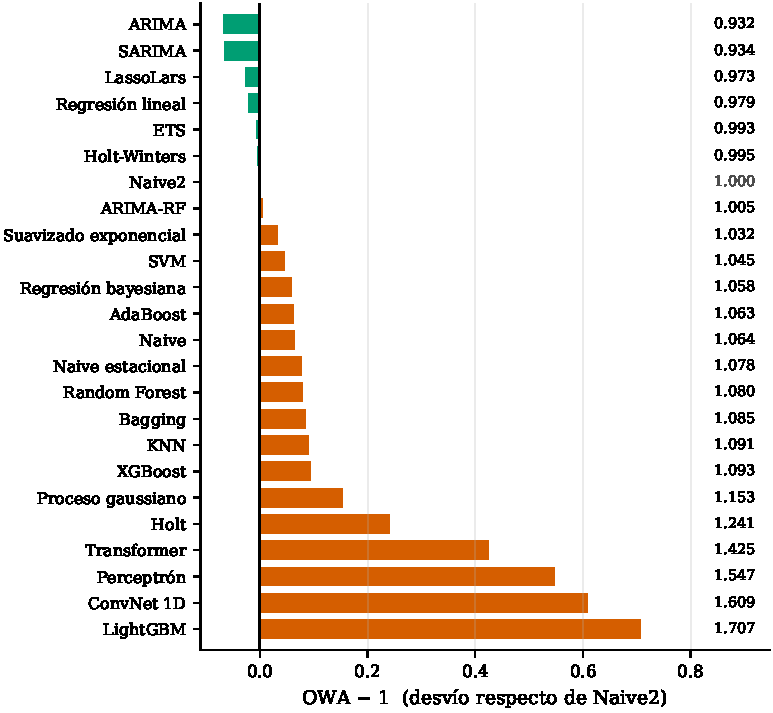
\includegraphics[width=0.72\linewidth]{figuras/fig6_owa_modelos.pdf}
\caption{Desvío del OWA respecto del benchmark Naive2. En verde los modelos que lo
superan; en gris el propio benchmark. Se omiten cuatro modelos con OWA $>3$ cuyos
promedios están dominados por ajustes divergentes (ver
Cuadro~\ref{tab:extremos}).}
\label{fig:owa}
\end{figure}
